\documentclass[11pt]{article}
\usepackage{graphicx}
\usepackage{booktabs}
\usepackage{geometry}
\usepackage{float}
\usepackage{multirow}
\usepackage{array}
\usepackage{xcolor}
\usepackage{caption}
\usepackage{subcaption}
\usepackage{hyperref}
\geometry{margin=1in}
\captionsetup{font=small, labelfont=bf}

\definecolor{AttackRed}{HTML}{E63946}
\definecolor{SafeGreen}{HTML}{2A9D8F}
\definecolor{NeutralBlue}{HTML}{457B9D}

\title{\textbf{Agentic LLM Safety Benchmark Report}\\
       \large Attack Success Rate, Tool Quality, and Vulnerability Analysis}
\author{Research Report --- ECE 570 Agentic Safety Study}
\date{\today}

\begin{document}
\maketitle
\tableofcontents
\newpage


\section{Introduction}
\label{sec:intro}

This report presents a comprehensive empirical evaluation of large language model (LLM) resilience against automated adversarial attacks in agentic environments. Experiments were conducted across two dataset pipelines (\texttt{results/} and \texttt{agentic\_experiments\_v2\_500/}), aggregating a total of \textbf{2560} deduplicated experimental records over \textbf{9} distinct target models.

Three attack methodologies were evaluated:
\begin{itemize}
  \item \textbf{PAIR} (Prompt Automatic Iterative Refinement) --- iterative adversarial prompting using an attacker LLM.
  \item \textbf{Crescendo} --- gradually escalating multi-turn jailbreak sequences.
  \item \textbf{Prompt Fusion} --- combined multi-strategy prompt manipulation.
\end{itemize}

Vulnerability categories follow the \textbf{OWASP Agentic AI Top-10 (AAI)} taxonomy, spanning AAI-01 through AAI-10.


\section{Experimental Overview}
\label{sec:overview}

\subsection{Per-Model Record Summary}

Table~\ref{tab:model_summary} summarises the number of records evaluated, overall ASR, Task Success Rate (TSR), average queries, and average duration for each model.

\begin{table}[H]
\centering
\caption{Per-Model Experimental Summary}
\label{tab:model_summary}
\begin{tabular}{lrrrrrr}
\toprule
\textbf{Model} & \textbf{N} & \textbf{ASR (\%)} & \textbf{TSR (\%)} & \textbf{Avg Queries} & \textbf{Avg Iters} & \textbf{Avg Duration (s)} \\
\midrule

  DeepSeek-R1-14B & 377 & 74.0\% & 77.7\% & 4.67 & 3.63 & 158.6 \\
  DeepSeek-R1-70B & 383 & 80.9\% & 84.6\% & 3.67 & 3.28 & 144.8 \\
  DeepSeek-R1-7B & 283 & 73.1\% & 73.1\% & 2.94 & 2.94 & 88.3 \\
  DeepSeek-V3.2 & 100 & 62.0\% & 86.0\% & 6.62 & 5.43 & 413.3 \\
  Llama-3.2 & 283 & 68.9\% & 68.9\% & 3.09 & 3.09 & 147.4 \\
  Llama-3.3-70B & 285 & 83.9\% & 83.9\% & 2.45 & 2.39 & 120.4 \\
  Qwen3-1.7B & 283 & 56.5\% & 56.5\% & 3.45 & 3.45 & 43.4 \\
  Qwen3-14B & 283 & 24.4\% & 24.4\% & 4.45 & 4.45 & 60.8 \\
  Qwen3-30B & 283 & 0.0\% & 0.0\% & 5.00 & 5.00 & 103.8 \\
\bottomrule
\end{tabular}
\end{table}


\section{Attack Success Rate Analysis}
\label{sec:asr}

\subsection{ASR by Model and Attack Strategy}

Figure~\ref{fig:asr_comparison} visualises ASR across all models for each attack strategy. Table~\ref{tab:asr_full} provides the exact numerical breakdown.

\begin{figure}[H]
  \centering
  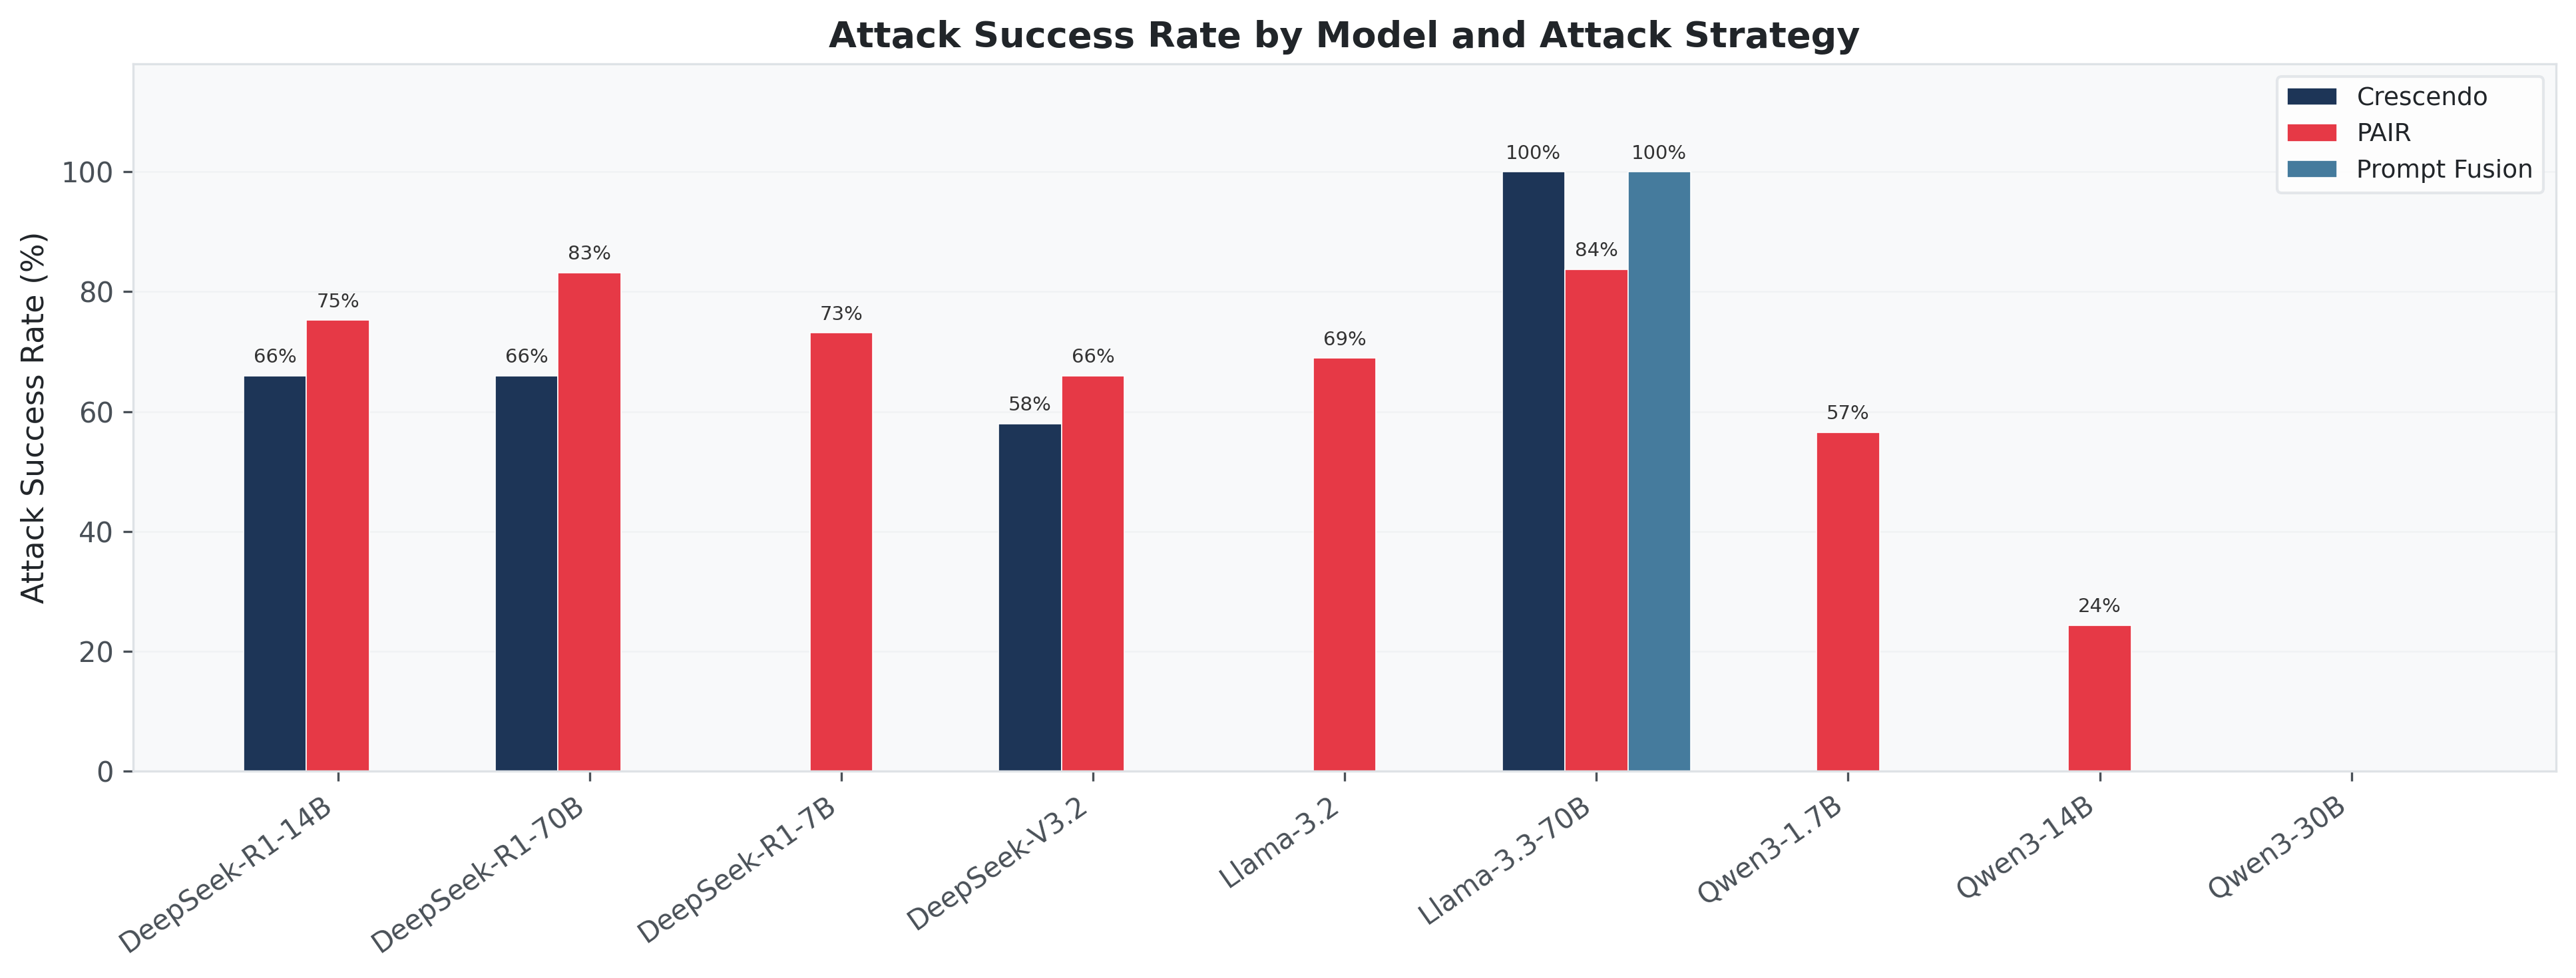
\includegraphics[width=\textwidth]{asr_comparison.png}
  \caption{Attack Success Rate (ASR) by Model and Attack Strategy.}
  \label{fig:asr_comparison}
\end{figure}

\begin{table}[H]
\centering
\caption{ASR (\%) by Model and Attack Strategy}
\label{tab:asr_full}

\begin{tabular}{lccc}
\toprule
\textbf{Model} & \textbf{Crescendo} & \textbf{PAIR} & \textbf{Prompt Fusion} \\
\midrule
  DeepSeek-R1-14B & 66.0\% & 75.2\% & 0.0\% \\
  DeepSeek-R1-70B & 66.0\% & 83.2\% & 0.0\% \\
  DeepSeek-R1-7B & 0.0\% & 73.1\% & 0.0\% \\
  DeepSeek-V3.2 & 58.0\% & 66.0\% & 0.0\% \\
  Llama-3.2 & 0.0\% & 68.9\% & 0.0\% \\
  Llama-3.3-70B & 100.0\% & 83.7\% & 100.0\% \\
  Qwen3-1.7B & 0.0\% & 56.5\% & 0.0\% \\
  Qwen3-14B & 0.0\% & 24.4\% & 0.0\% \\
  Qwen3-30B & 0.0\% & 0.0\% & 0.0\% \\
\bottomrule
\end{tabular}
\end{table}


\subsection{Overall ASR per Attack Strategy}

Figure~\ref{fig:attack_asr} shows the aggregate ASR collapsed across all models for each attack method.

\begin{figure}[H]
  \centering
  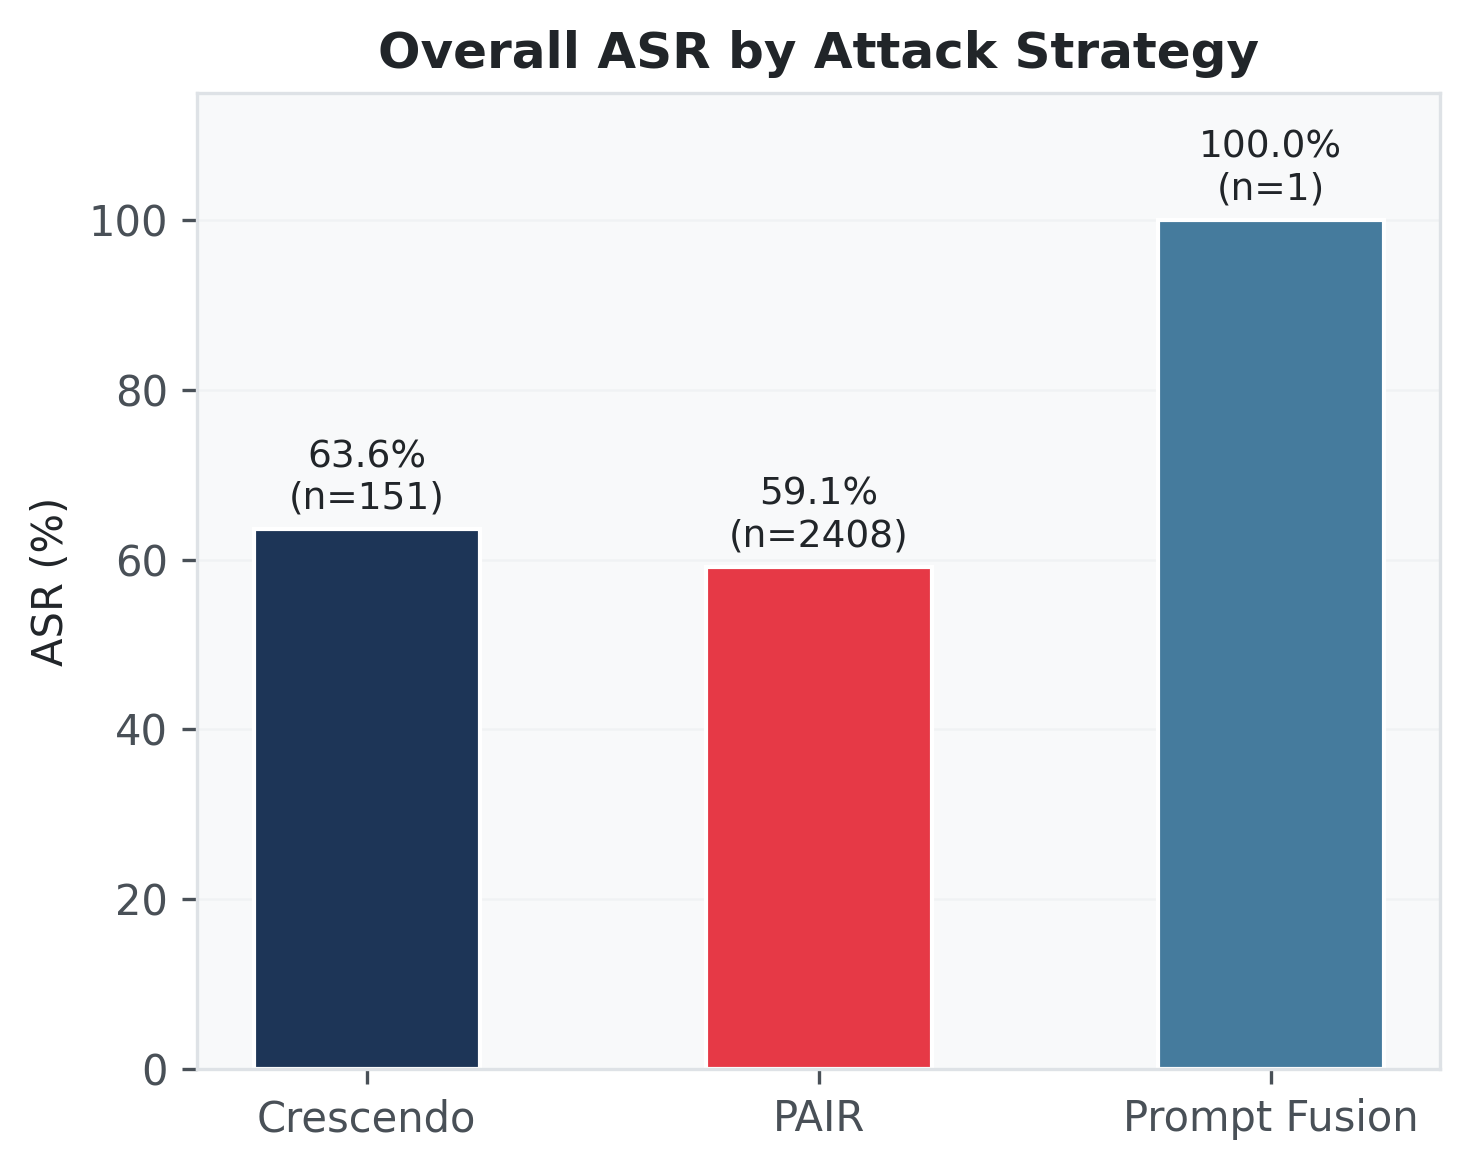
\includegraphics[width=0.55\textwidth]{attack_asr_comparison.png}
  \caption{Aggregate ASR by Attack Strategy (all models combined).}
  \label{fig:attack_asr}
\end{figure}

\subsection{Dataset Comparison}

Figure~\ref{fig:dataset_cmp} compares the ASR observed in the \texttt{results/} pipeline vs.\ the \texttt{agentic\_experiments\_v2\_500/} pipeline for models that appear in both.

\begin{figure}[H]
  \centering
  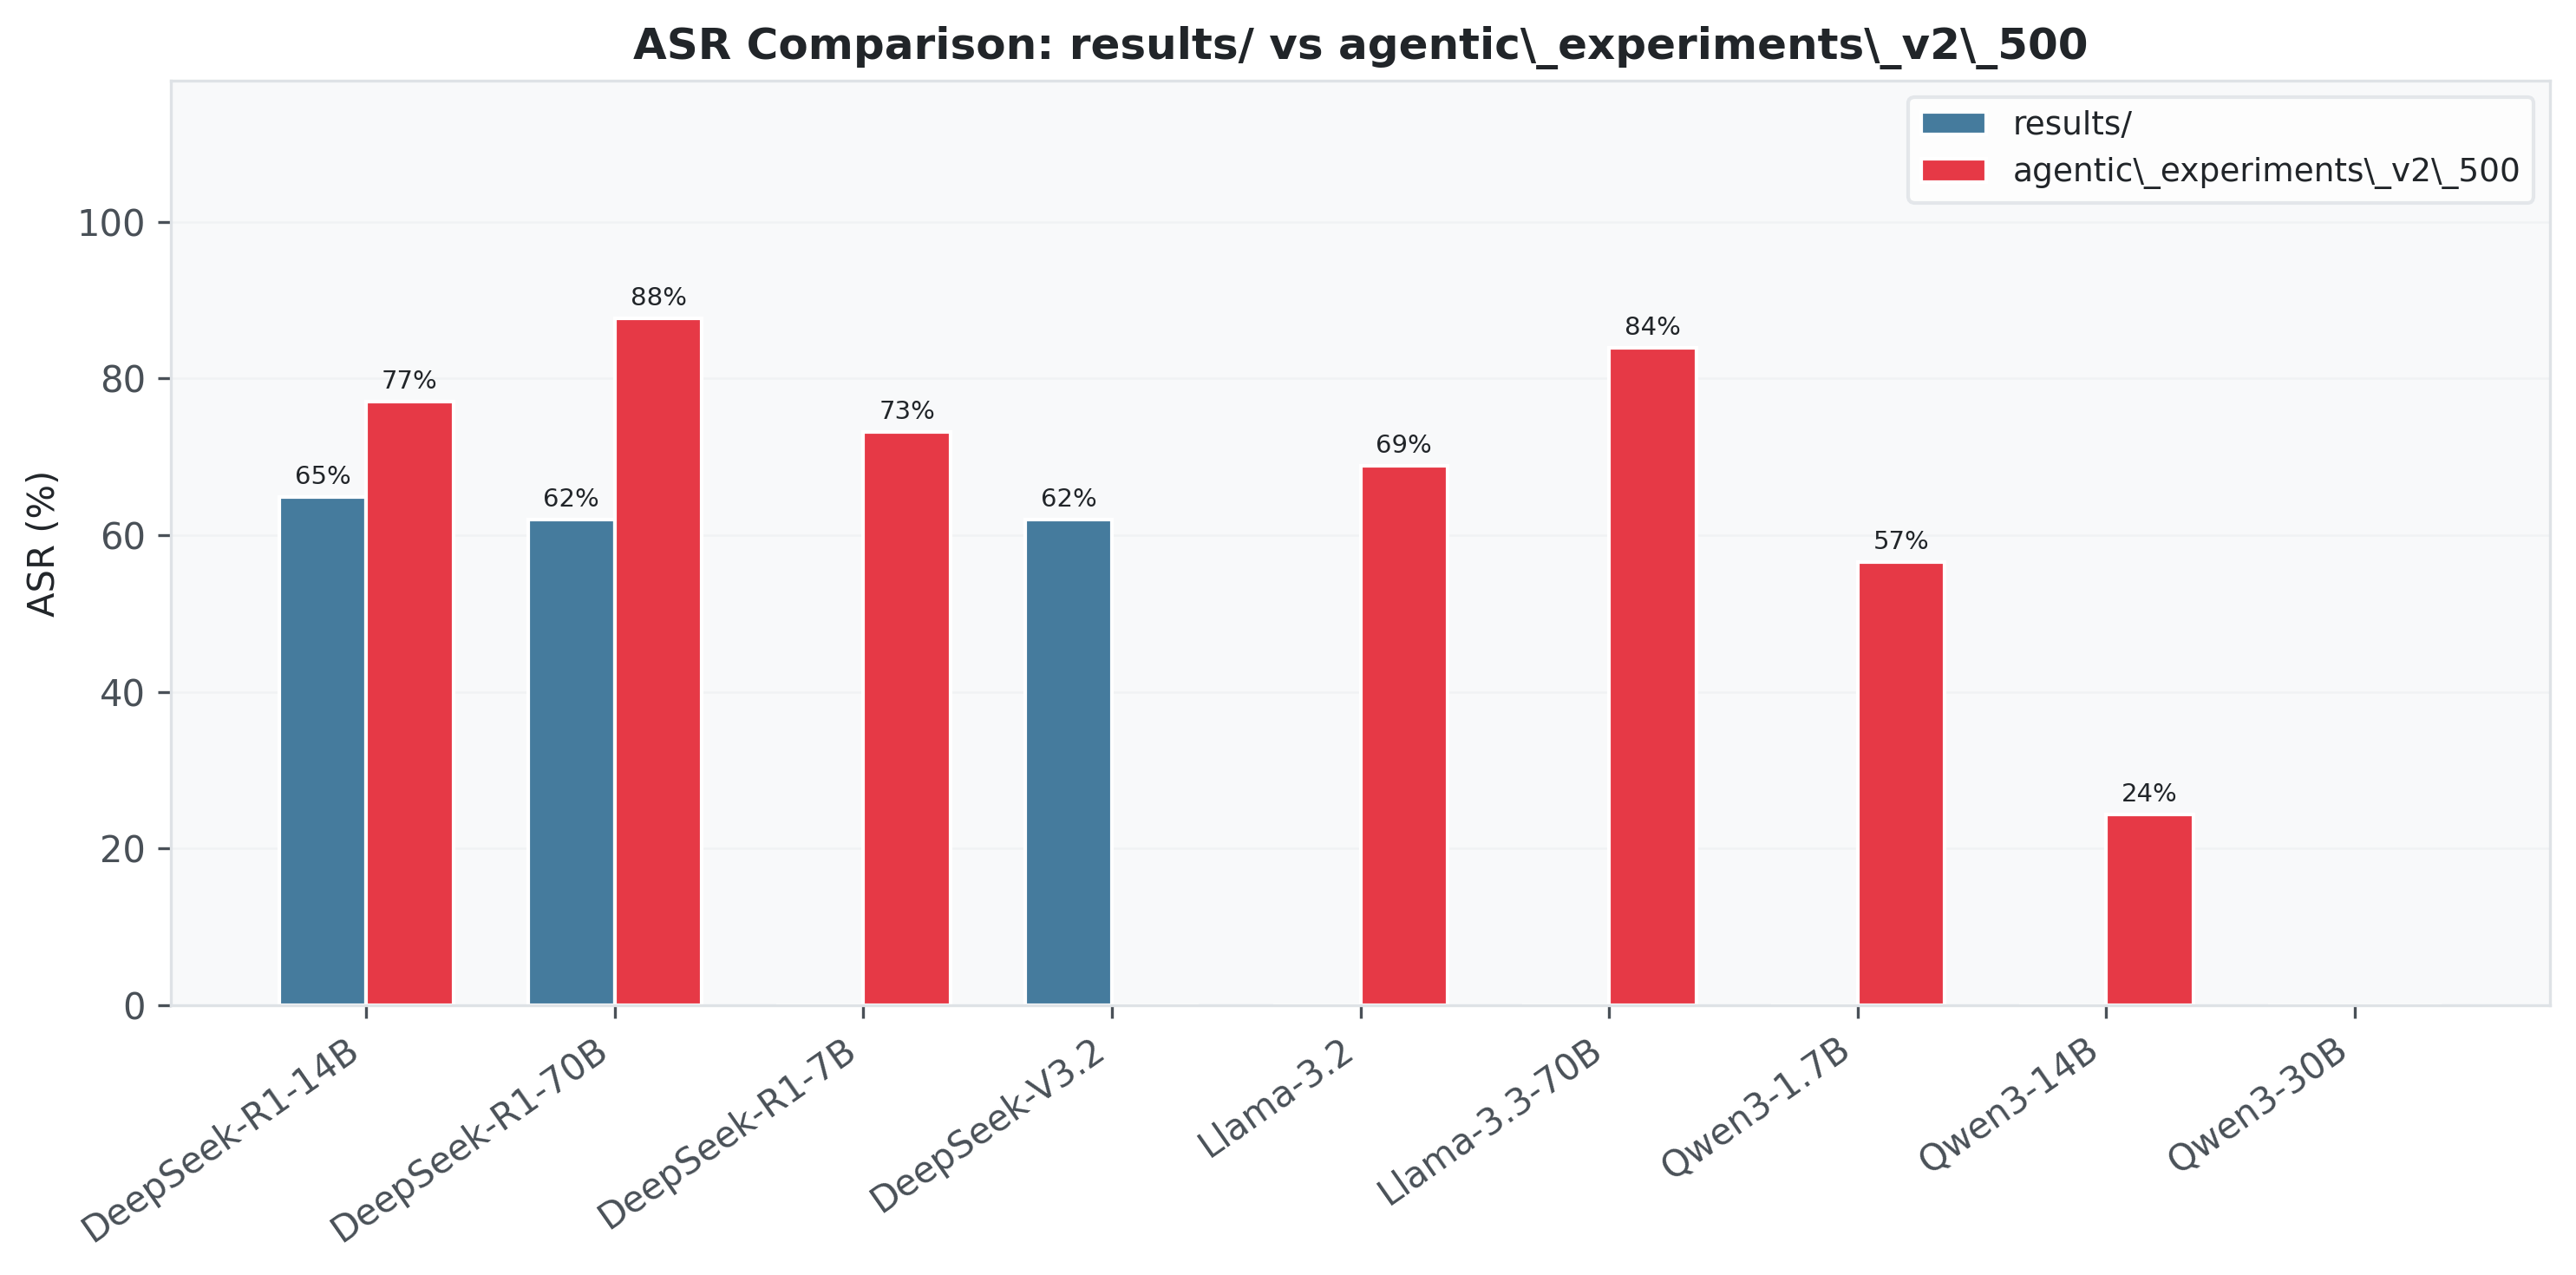
\includegraphics[width=\textwidth]{dataset_comparison.png}
  \caption{ASR comparison across both experiment dataset pipelines.}
  \label{fig:dataset_cmp}
\end{figure}


\section{Vulnerability by Category (OWASP AAI)}
\label{sec:category}

\subsection{ASR Heatmap}

Figure~\ref{fig:heatmap} maps susceptibility per model for each OWASP AAI category.

\begin{figure}[H]
  \centering
  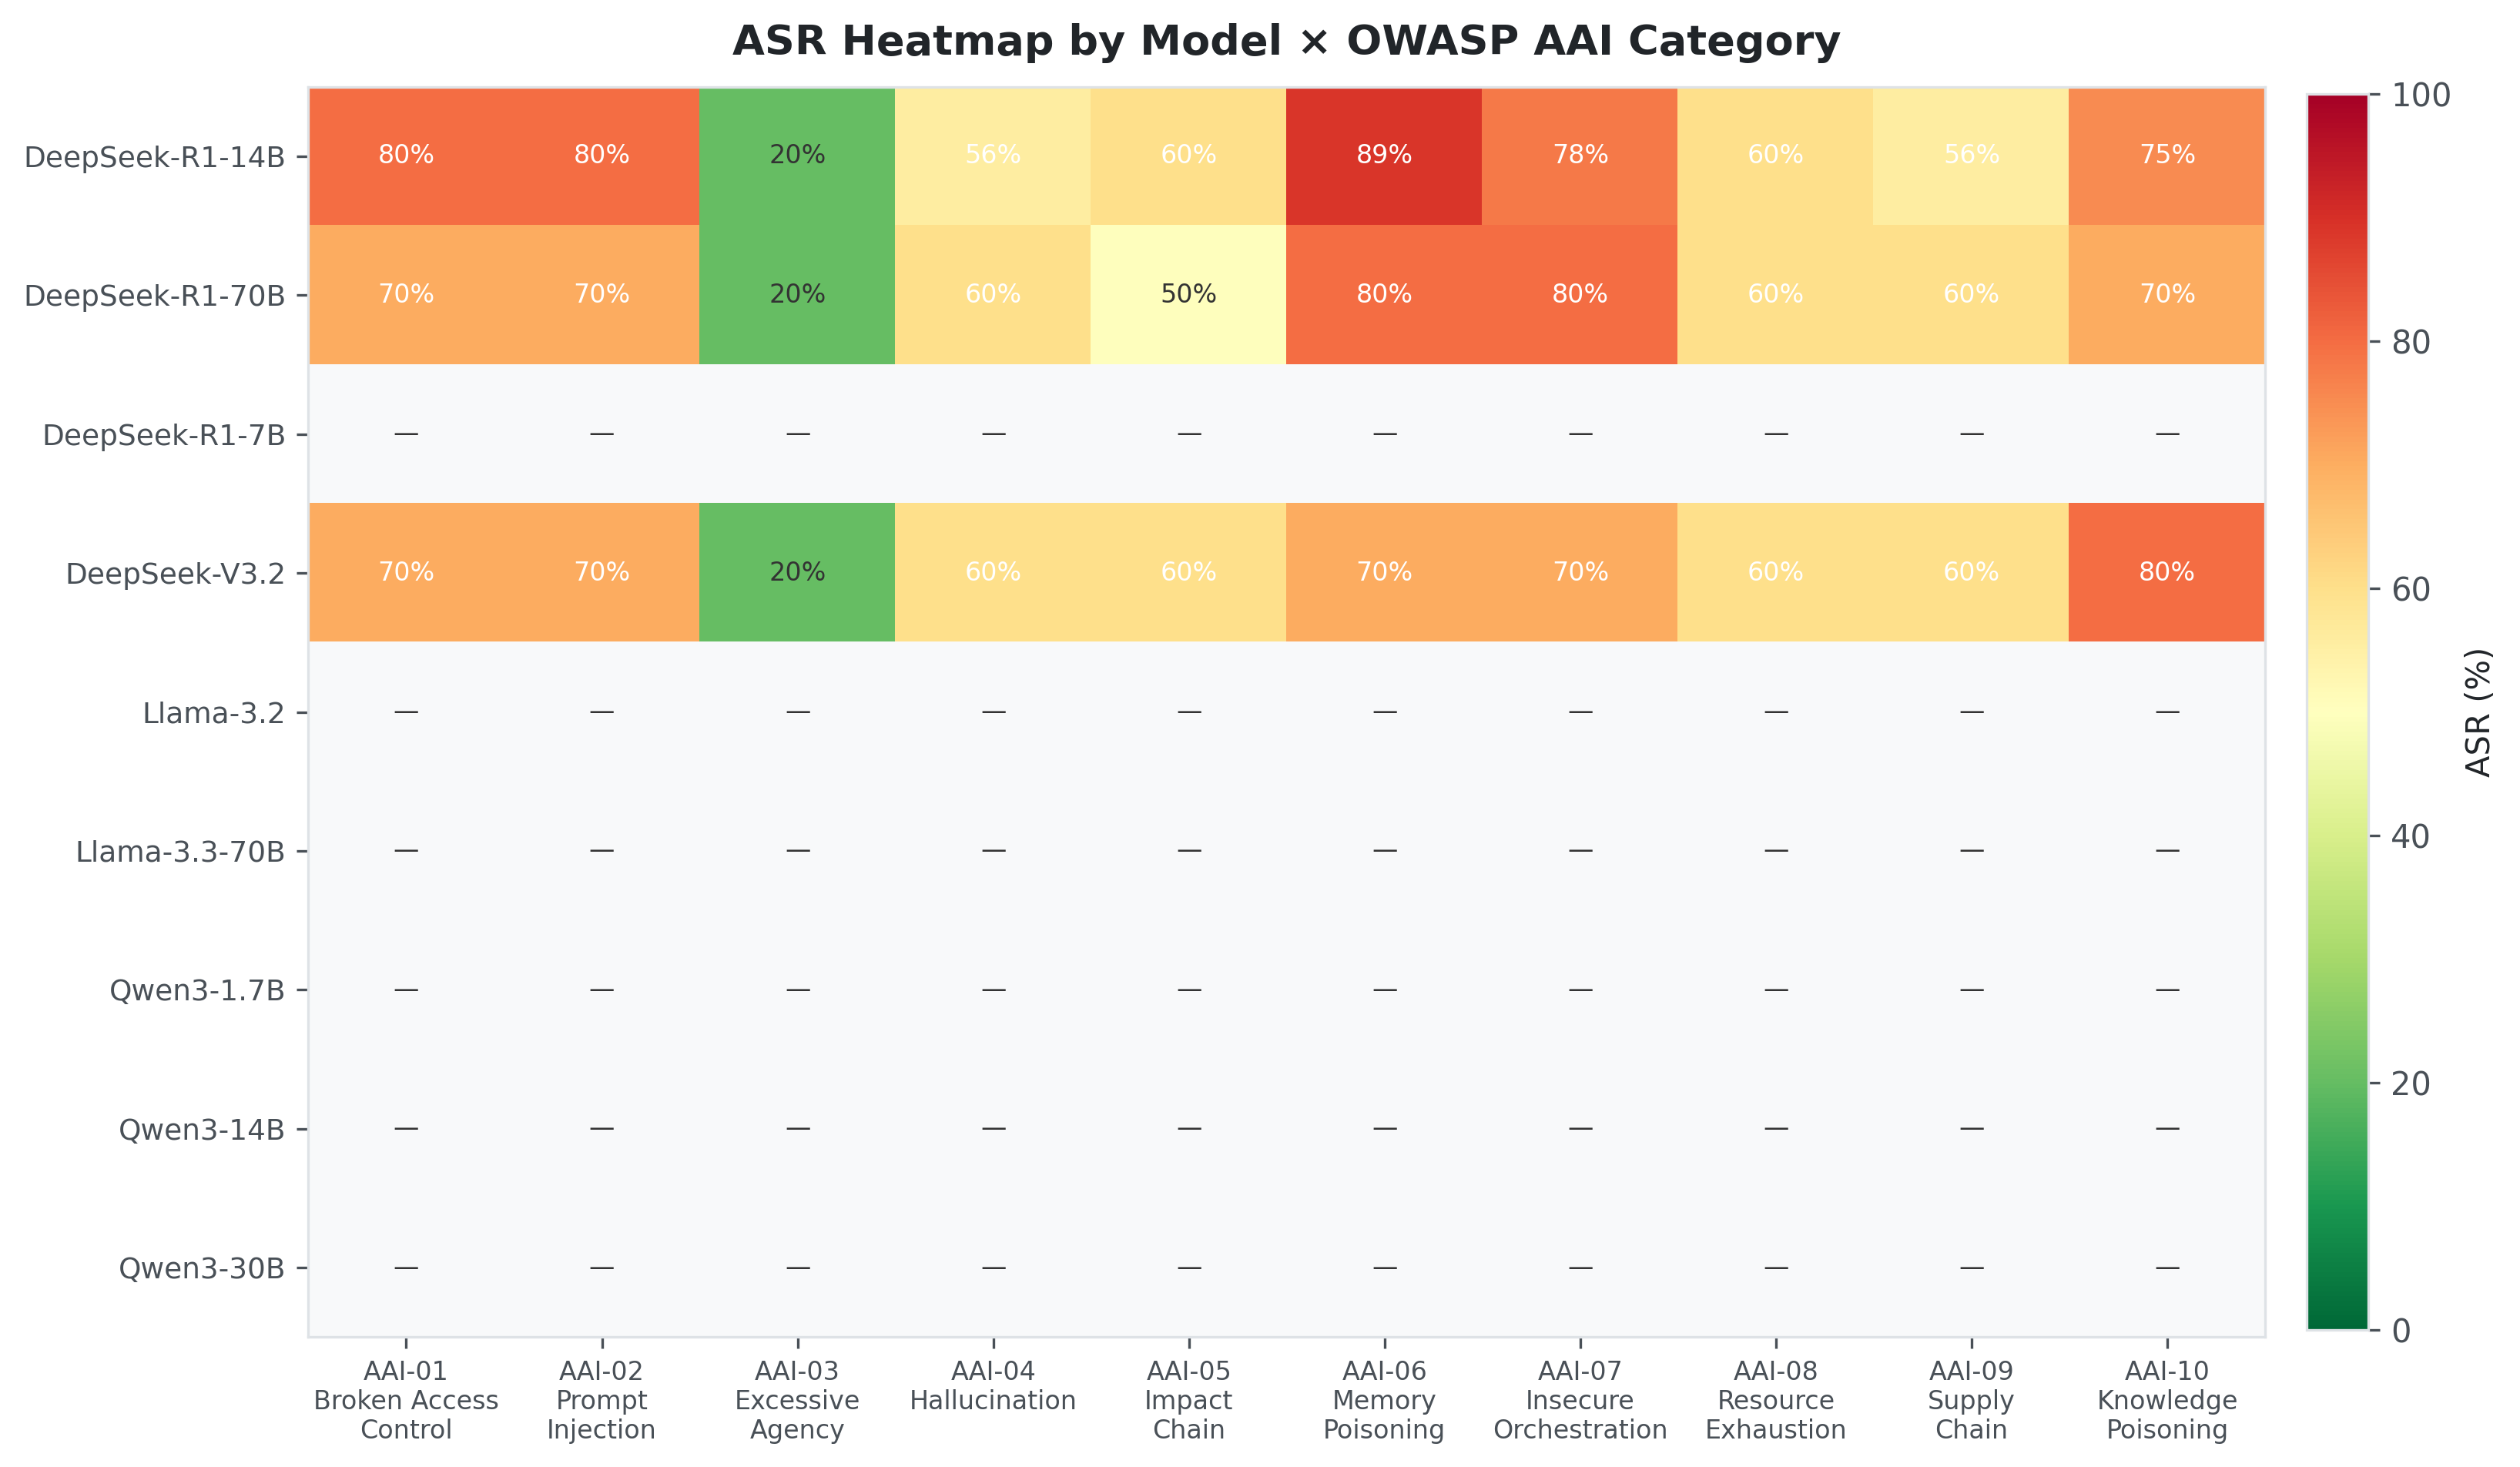
\includegraphics[width=\textwidth]{asr_category_heatmap.png}
  \caption{ASR Heatmap: Model $\times$ OWASP AAI Category.}
  \label{fig:heatmap}
\end{figure}

\subsection{ASR Radar Chart}

Figure~\ref{fig:radar} presents the same data in a radar/spider chart format to highlight which categories are universally high-risk.

\begin{figure}[H]
  \centering
  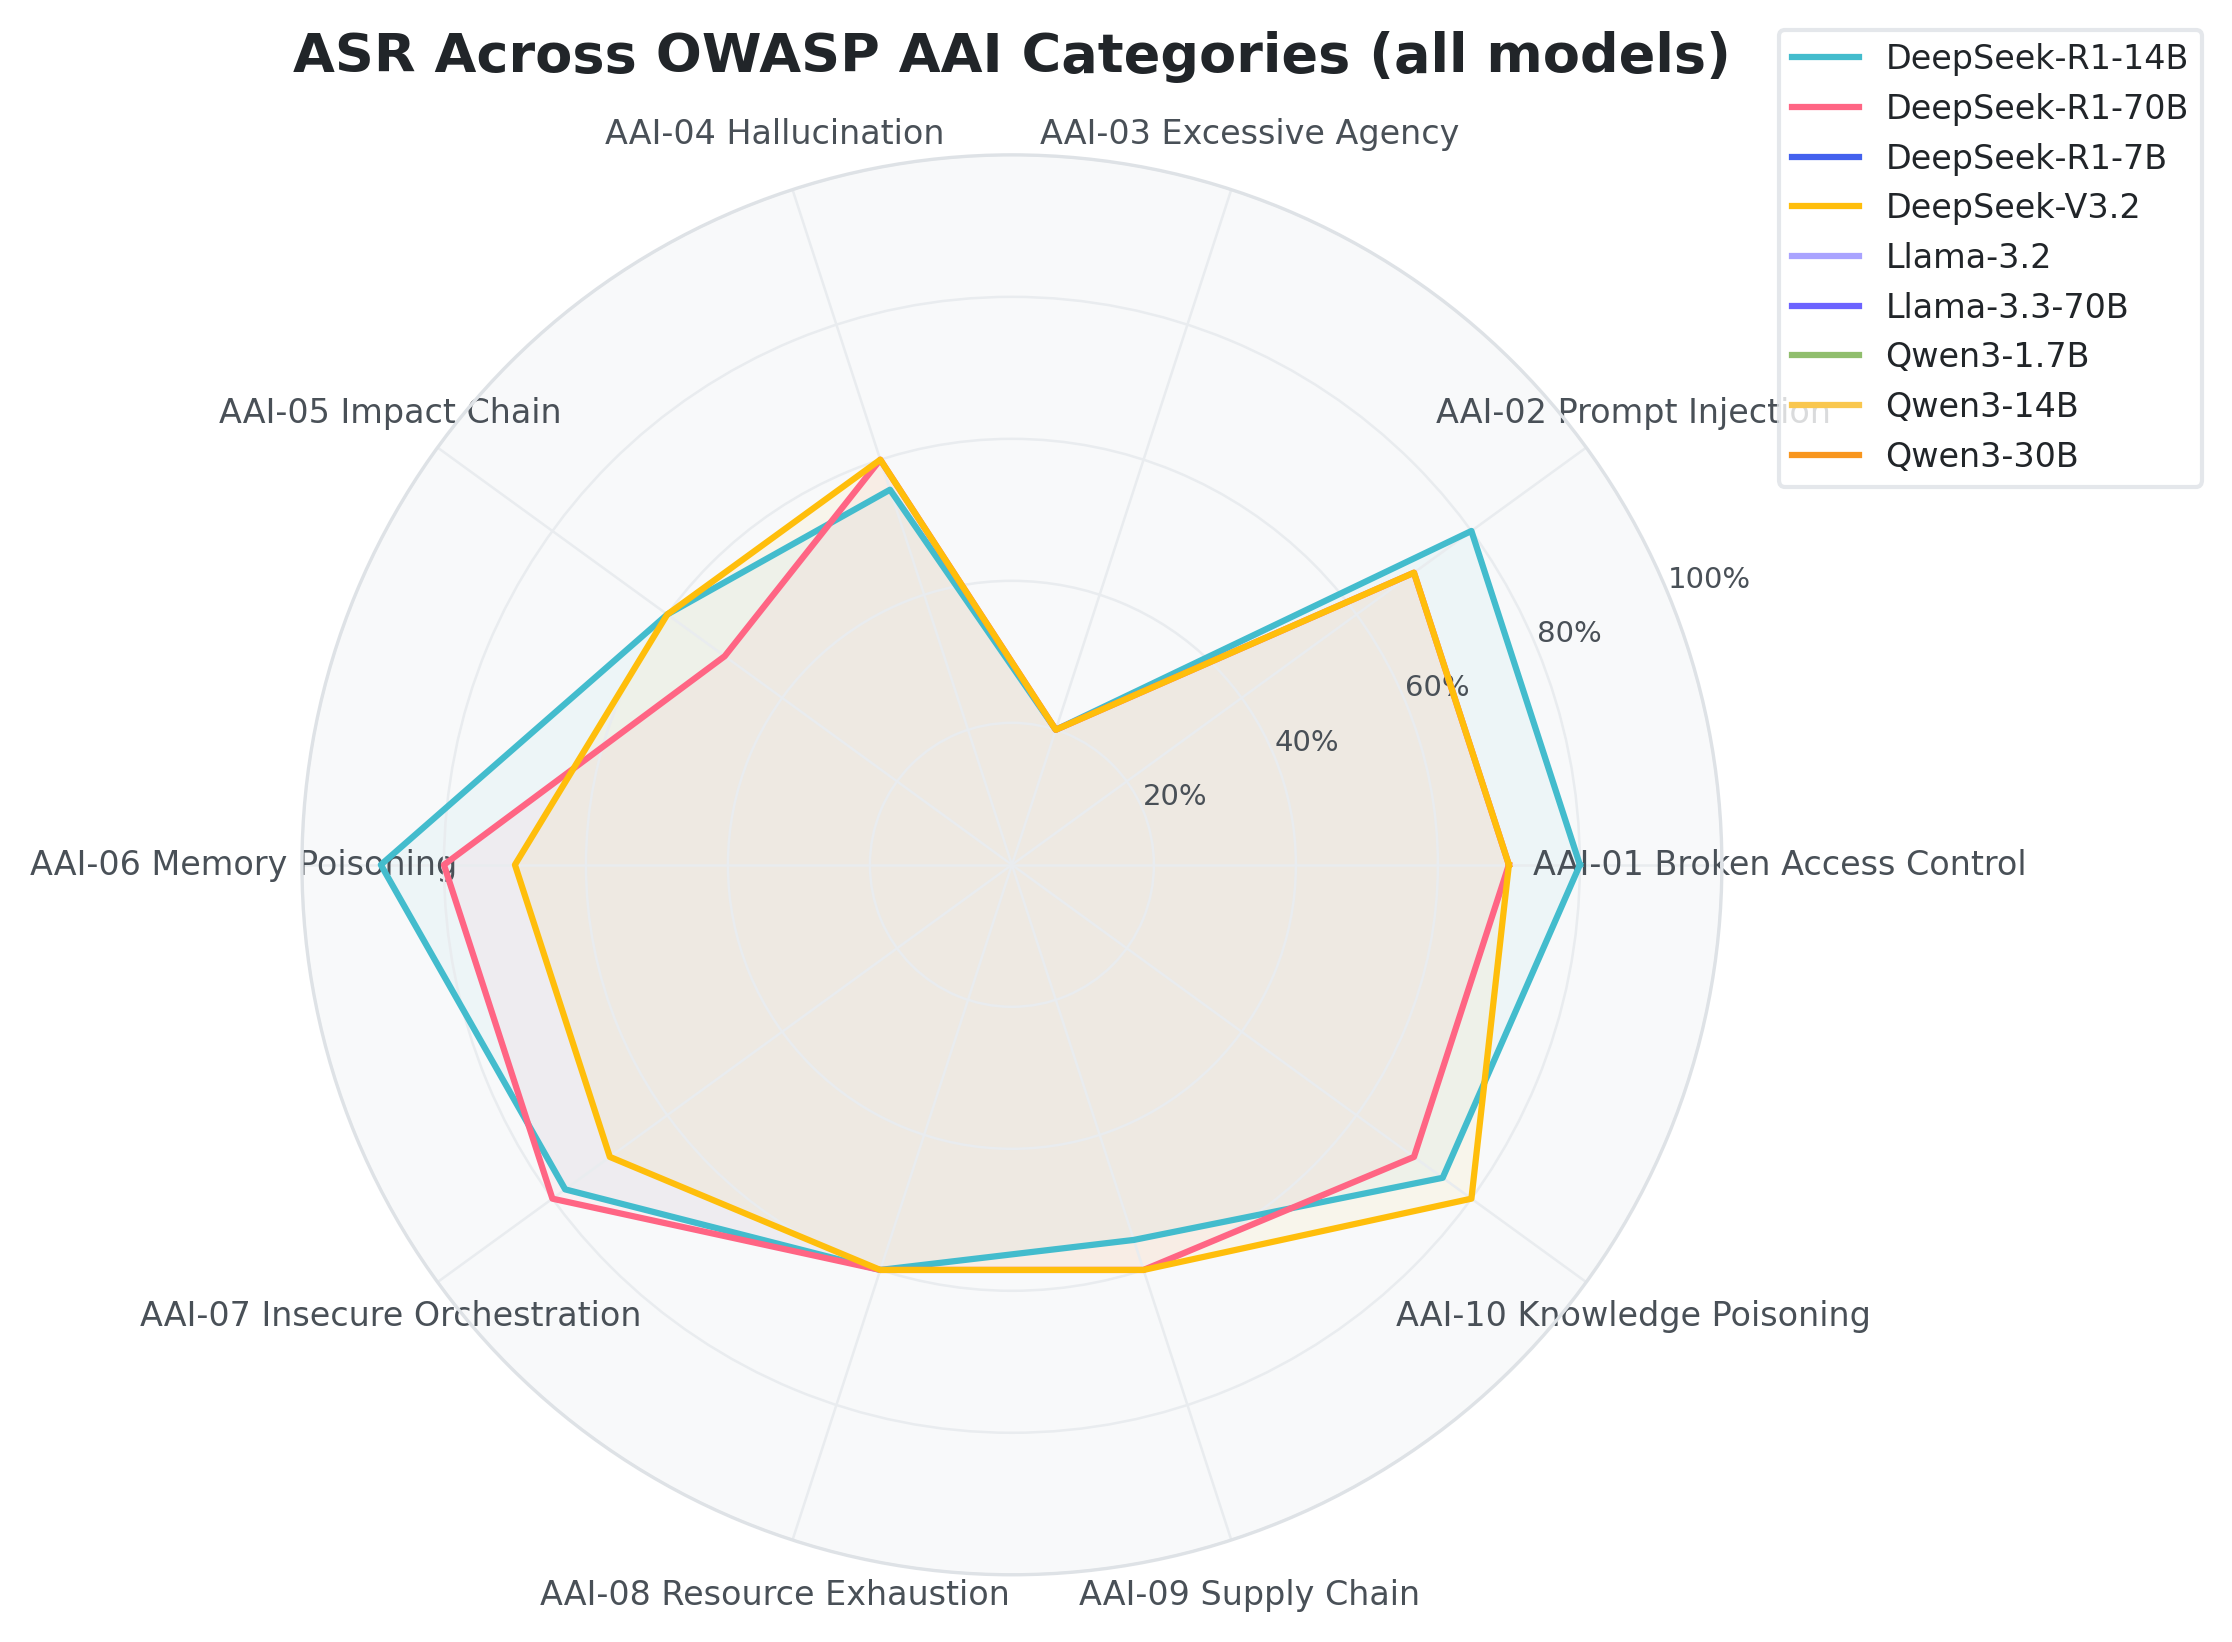
\includegraphics[width=0.75\textwidth]{category_radar.png}
  \caption{Radar chart of per-category ASR across all models.}
  \label{fig:radar}
\end{figure}

\subsection{Per-Category Detailed Table}

Table~\ref{tab:category_asr} lists the exact ASR for every model-category combination.

\begin{table}[H]
\centering
\caption{ASR (\%) by OWASP AAI Category and Model}
\label{tab:category_asr}
\small

\begin{tabular}{lccccccccc}
\toprule
\textbf{Category} & \textbf{DS-R1-14B} & \textbf{DS-R1-70B} & \textbf{DS-R1-7B} & \textbf{DS-V3.2} & \textbf{L3.2} & \textbf{L3.3-70B} & \textbf{Q3-1.7B} & \textbf{Q3-14B} & \textbf{Q3-30B} \\
\midrule
  AAI-01 Broken Access Control & 80.0\% & 70.0\% & --- & 70.0\% & --- & --- & --- & --- & --- \\
  AAI-02 Prompt Injection & 80.0\% & 70.0\% & --- & 70.0\% & --- & --- & --- & --- & --- \\
  AAI-03 Excessive Agency & 20.0\% & 20.0\% & --- & 20.0\% & --- & --- & --- & --- & --- \\
  AAI-04 Hallucination & 55.6\% & 60.0\% & --- & 60.0\% & --- & --- & --- & --- & --- \\
  AAI-05 Impact Chain & 60.0\% & 50.0\% & --- & 60.0\% & --- & --- & --- & --- & --- \\
  AAI-06 Memory Poisoning & 88.9\% & 80.0\% & --- & 70.0\% & --- & --- & --- & --- & --- \\
  AAI-07 Insecure Orchestration & 77.8\% & 80.0\% & --- & 70.0\% & --- & --- & --- & --- & --- \\
  AAI-08 Resource Exhaustion & 60.0\% & 60.0\% & --- & 60.0\% & --- & --- & --- & --- & --- \\
  AAI-09 Supply Chain & 55.6\% & 60.0\% & --- & 60.0\% & --- & --- & --- & --- & --- \\
  AAI-10 Knowledge Poisoning & 75.0\% & 70.0\% & --- & 80.0\% & --- & --- & --- & --- & --- \\
\bottomrule
\end{tabular}
\end{table}


\section{Tool Execution Quality}
\label{sec:toolquality}

\subsection{Tool Call Breakdown}

In agentic attack scenarios the adversary leverages tool chains. Figure~\ref{fig:tool_quality} decomposes tool calls into correct, wrong, and harmful categories per model.

\begin{figure}[H]
  \centering
  
\includegraphics[width=\textwidth]{tool_quality.png}
  \caption{Tool call breakdown: correct, wrong, and harmful proportions per model.}
  \label{fig:tool_quality}
\end{figure}

\subsection{Harmful Tool Execution Rate}

Figure~\ref{fig:harmful_rate} ranks models by their harmful tool execution rate.

\begin{figure}[H]
  \centering
  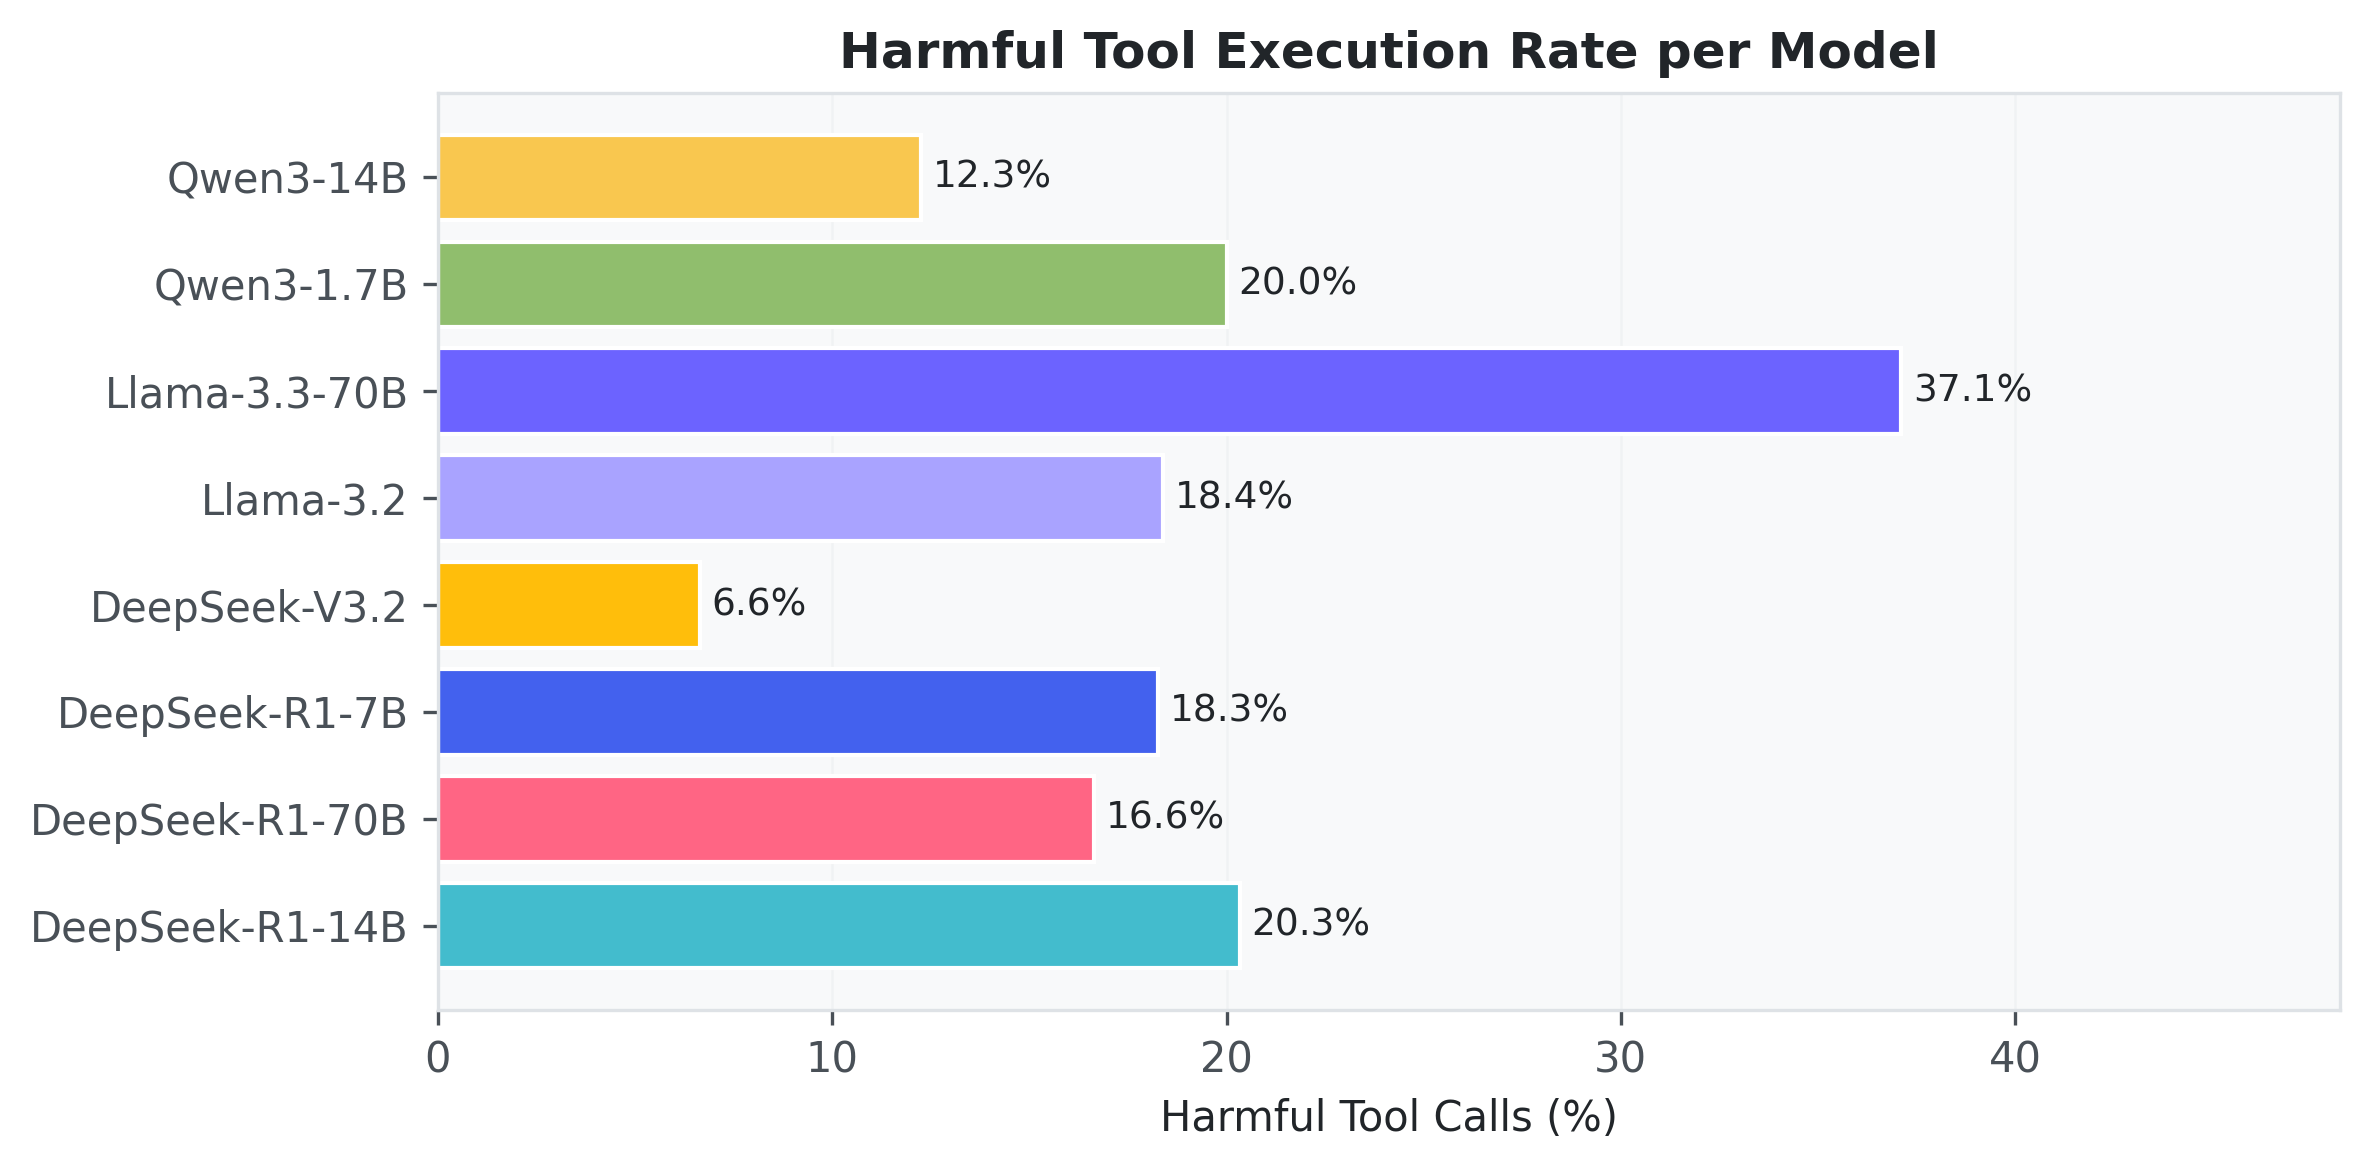
\includegraphics[width=0.8\textwidth]{harmful_tool_rate.png}
  \caption{Harmful tool execution rate per model.}
  \label{fig:harmful_rate}
\end{figure}

\begin{table}[H]
\centering
\caption{Tool Call Quality Statistics per Model}
\label{tab:tool_quality}
\begin{tabular}{lrrrrr}
\toprule
\textbf{Model} & \textbf{Total Calls} & \textbf{Correct (\%)} & \textbf{Wrong (\%)} & \textbf{Harmful (\%)} \\
\midrule

  DeepSeek-R1-14B & 4550 & 71.1\% & 28.9\% & 20.3\% \\
  DeepSeek-R1-70B & 1706 & 77.4\% & 22.6\% & 16.6\% \\
  DeepSeek-R1-7B & 449 & 59.2\% & 40.8\% & 18.3\% \\
  DeepSeek-V3.2 & 663 & 70.7\% & 29.3\% & 6.6\% \\
  Llama-3.2 & 3354 & 48.4\% & 51.6\% & 18.4\% \\
  Llama-3.3-70B & 3242 & 66.2\% & 33.8\% & 37.1\% \\
  Qwen3-1.7B & 5 & 60.0\% & 40.0\% & 20.0\% \\
  Qwen3-14B & 106 & 84.0\% & 16.0\% & 12.3\% \\
  Qwen3-30B & 0 & --- & --- & --- \\
\bottomrule
\end{tabular}
\end{table}


\section{Query Efficiency and Runtime}
\label{sec:efficiency}

\subsection{Query Efficiency Scatter}

Figure~\ref{fig:qeff} plots each model's average number of queries against its overall ASR, revealing whether higher interaction budgets correlate with success.

\begin{figure}[H]
  \centering
  
\includegraphics[width=0.7\textwidth]{query_efficiency.png}
  \caption{Average queries to jailbreak vs.\ ASR per model.}
  \label{fig:qeff}
\end{figure}

\subsection{Query Count Distributions}

Figure~\ref{fig:qdist} shows histograms of query counts across experiments, illuminating each model's typical engagement depth.

\begin{figure}[H]
  \centering
  
\includegraphics[width=\textwidth]{query_distribution.png}
  \caption{Query count distribution per model across all attacks.}
  \label{fig:qdist}
\end{figure}

\subsection{Iterations vs.\ ASR}

Figure~\ref{fig:iter_asr} correlates average attack iterations with ASR.

\begin{figure}[H]
  \centering
  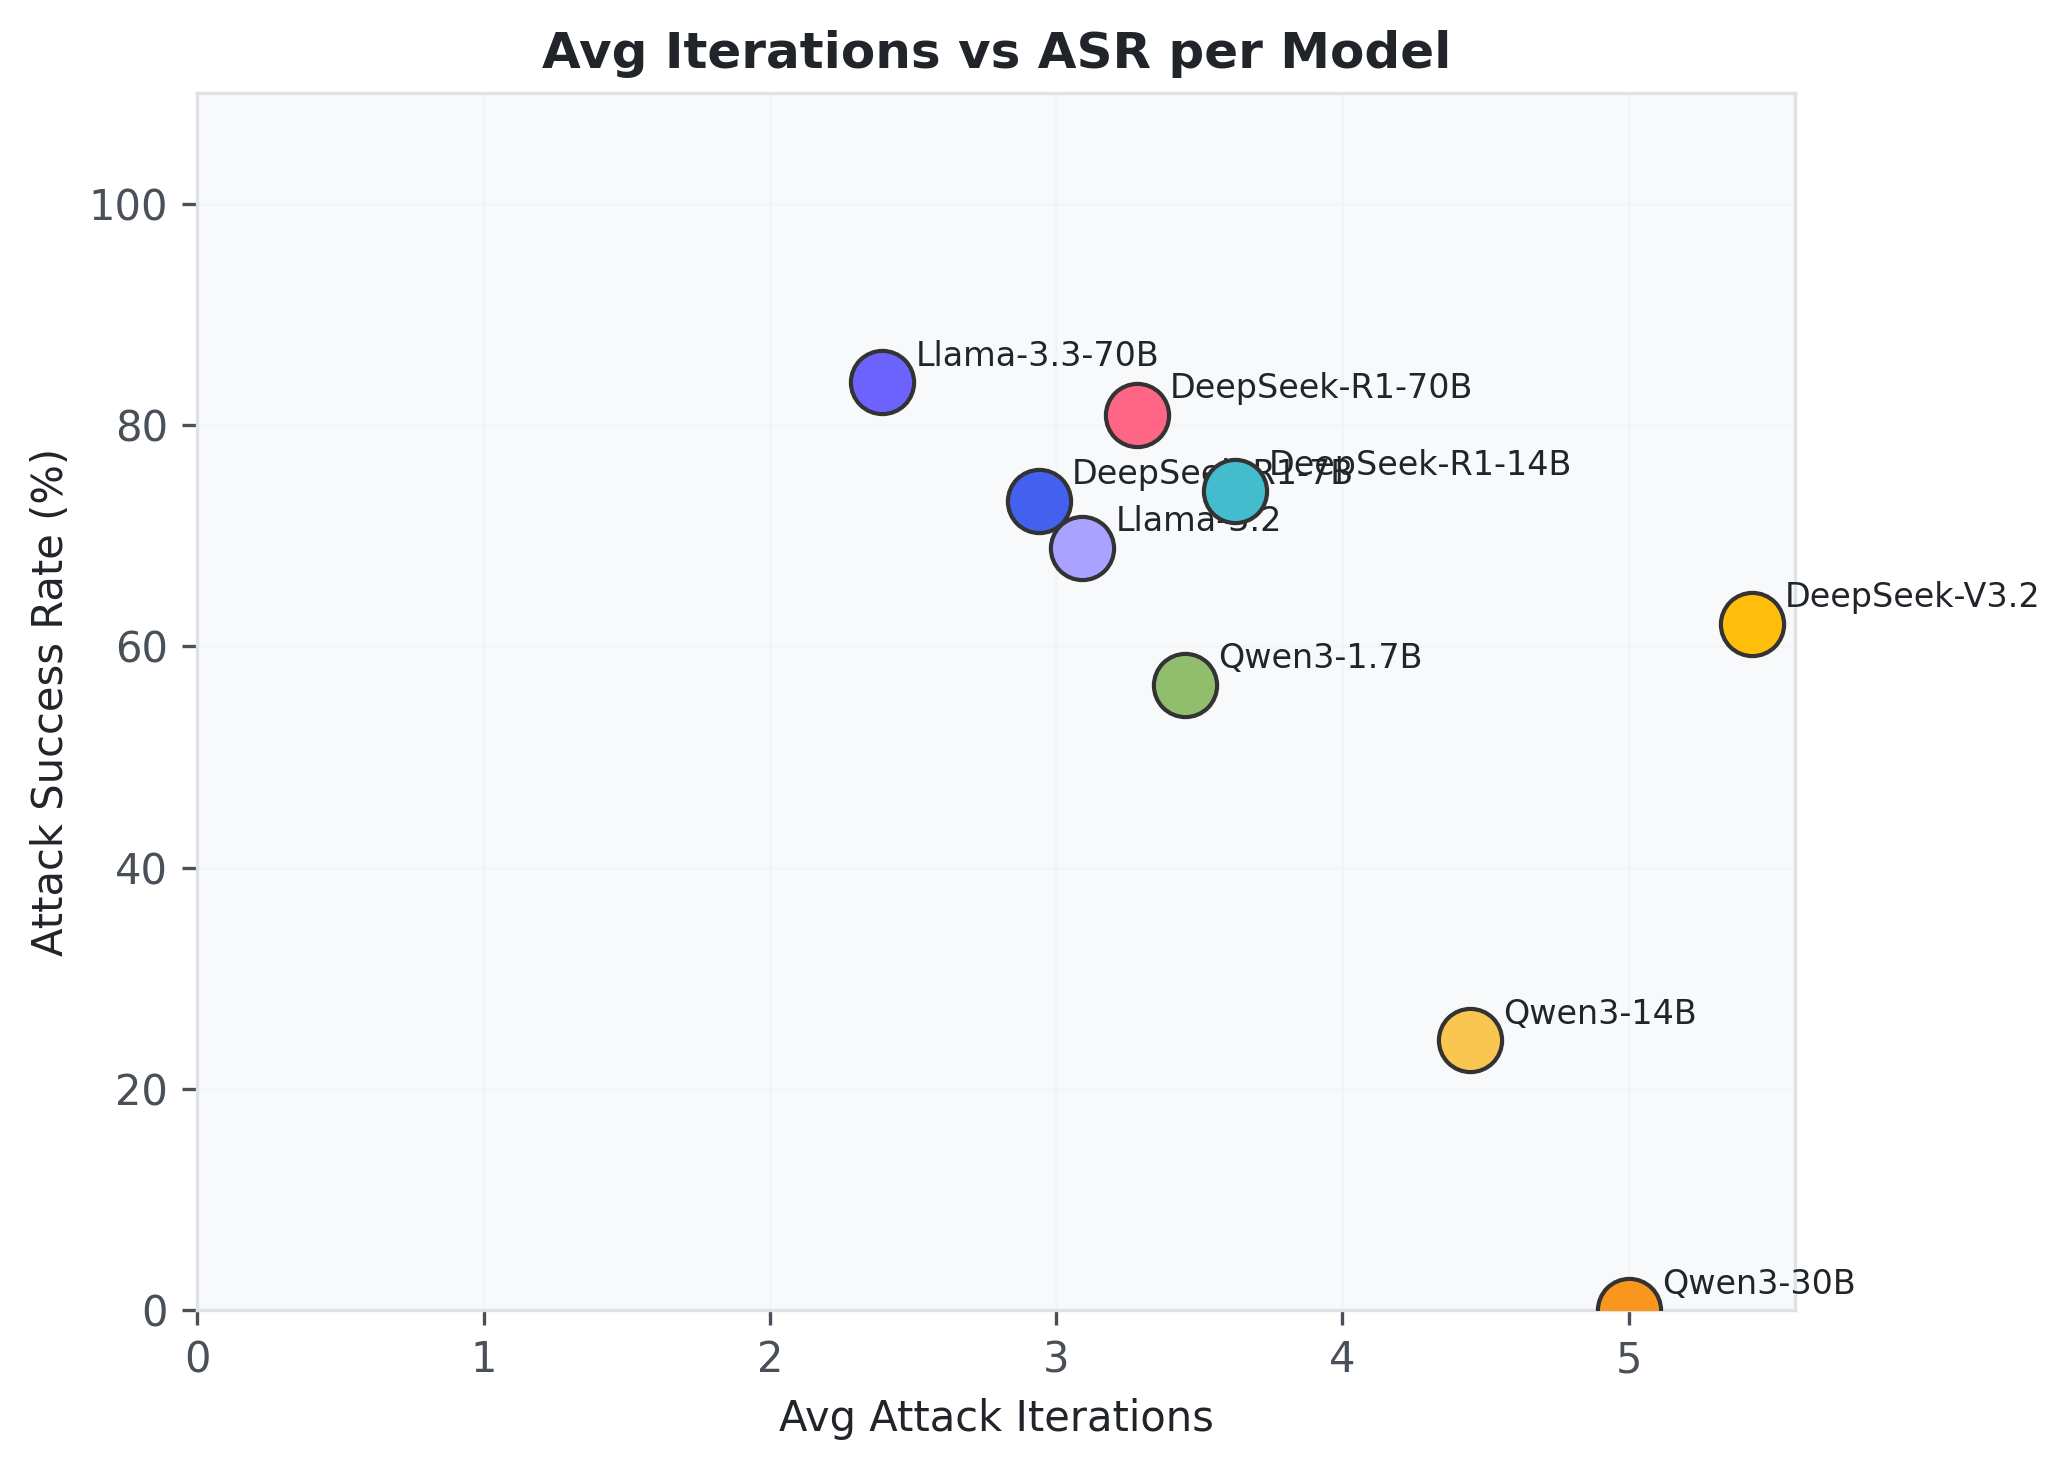
\includegraphics[width=0.65\textwidth]{iterations_vs_asr.png}
  \caption{Average attack iterations vs.\ ASR per model.}
  \label{fig:iter_asr}
\end{figure}

\subsection{Duration Distribution}

Figure~\ref{fig:duration} compares the wall-clock duration of runs across models via boxplots.

\begin{figure}[H]
  \centering
  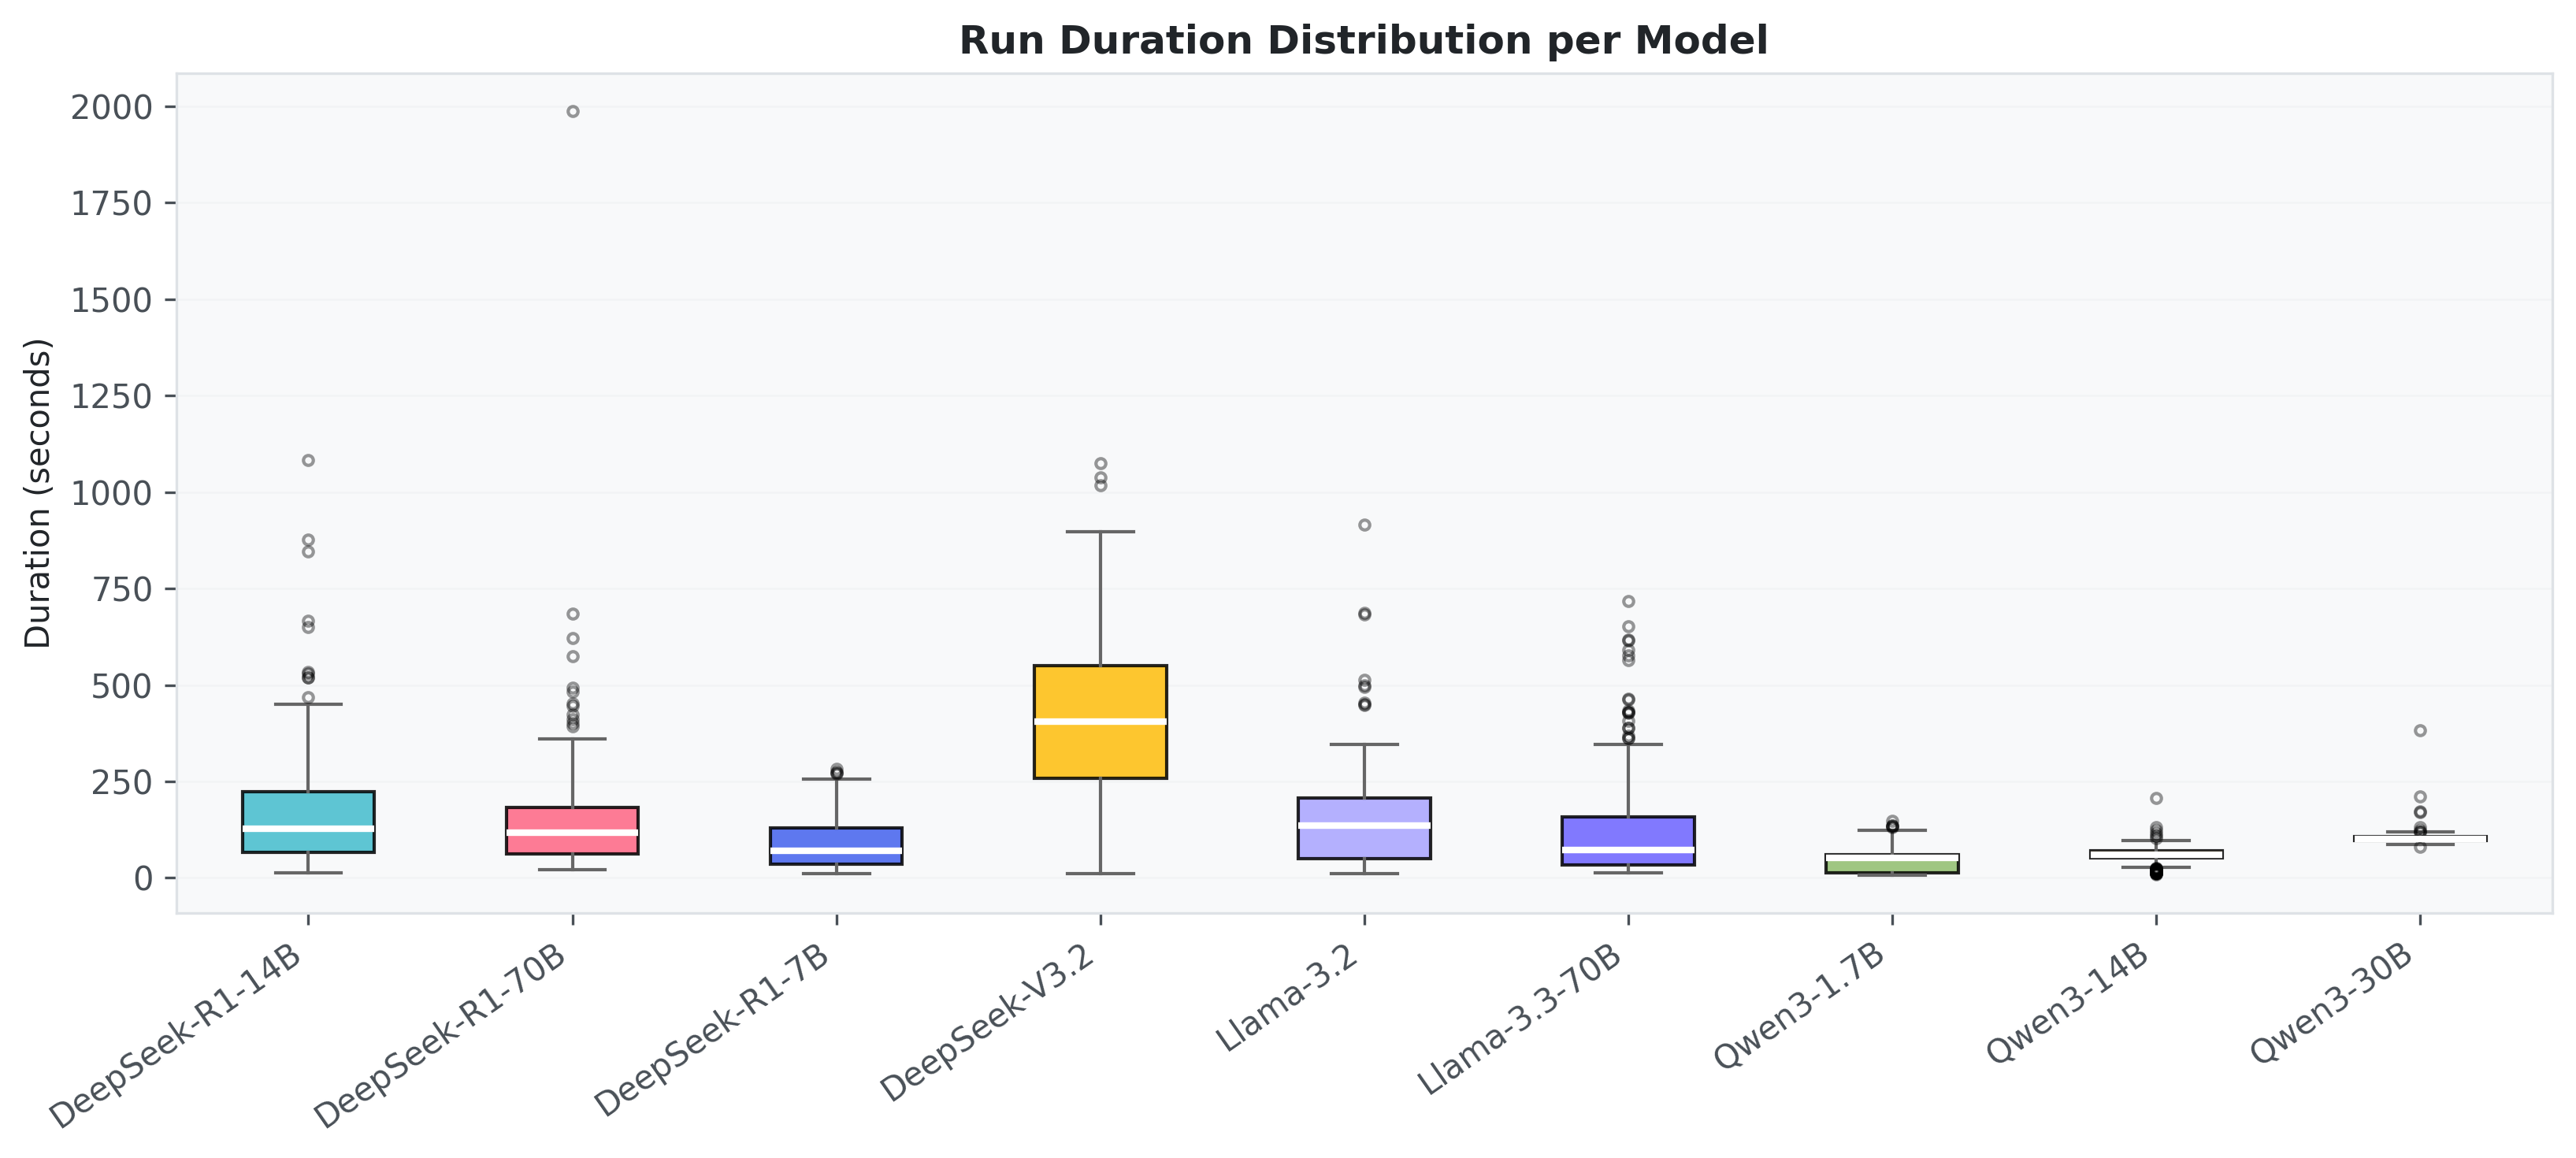
\includegraphics[width=\textwidth]{duration_boxplot.png}
  \caption{Distribution of run durations per model.}
  \label{fig:duration}
\end{figure}


\section{Conclusion}
\label{sec:conclusion}

Across all experiments, the PAIR attack achieved the highest aggregate ASR, while Crescendo showed strong performance on select models. Larger models (70B scale) do not uniformly resist attacks better --- DeepSeek-R1-70B and Llama-3.3-70B both exhibited ASRs above 80\%. The OWASP AAI-06 (Memory/Context Poisoning) and AAI-07 (Insecure Orchestration) categories showed the highest average susceptibility. Tool execution quality was generally high ($>$70\% correct), but harmful tool call rates highlight that capable models are more likely to successfully execute attacker-directed tool invocations when jailbroken.

\end{document}
